\subsection{Mathematical Modeling and Engineering Problem Solving - Chapter 1}

\begin{enumerate}

  \item {\bf General Formulation of Engineering Problems}
    The general formulation of an engineering problem has 4
    parts. Problem Definition, Mathematical Model, Computer Code and
    Implementation. The flow of the steps is shown in the figure
    below. Notice that determining the Mathematical Model involves
    Theory and Data.
    \begin{figure}[htb]
      \begin{center}
        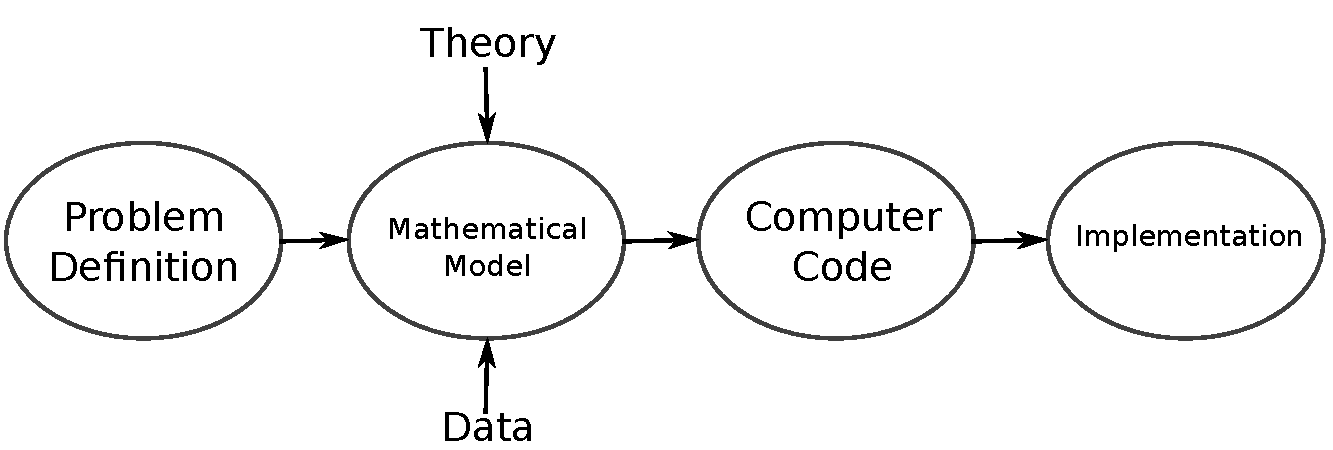
\includegraphics[height=0.25\textwidth,width=0.65\textwidth]{Graphics/Engineering_Problem.pdf}
      \end{center}
    \end{figure}
    Every problem starts with the definition of a problem. Using this
    problem a mathematical model is created to solve the problem. This
    mathematical model will require data and theory. Using this
    mathematical model a computer tool will be created. The code is
    then implemented to analyze the problem defined and make decisions
    based on the output of the model. 
    
  \item {\bf Example Problem}

    Problem Definition: How do I get on top of my roof? 

    Mathematical Model is the angle of the Ladder.
    
    Problem Definition: A round ball is launched straight into the
    air. The initial velocity, mass and initial height are given. If
    air drag is neglected what is the maximum height of the ball and
    what is the final time before it hits the ground.

    The mathematical model is this case takes the form

    \begin{equation}\nonumber
      Dependent~variable=f(independent~variable,parameters,forcing~function)
    \end{equation}

    In the example above our independent variable is time. The
    parameters are $v_0$,$m$, and $y_0$. These are the initial
    velocity, mass and height of the ball. The forcing function is
    gravity or $-mg$. The theory associated with this system is
    Newton's equation of motion and the data are the givens. Here
    Newton's equation of motion can be solved to obtain the height of
    the ball at time t.

    \begin{equation}
      y(t) = y_0 + v_0t - (1/2)gt^2
    \end{equation}

    A computer tool can be used to plot the location of the ball as a
    function of time. The code can then be implemented in order to
    obtain the maximum height of the ball and the time the ball hits
    the ground.

  \item {\bf False Assumptions}

    John takes $T_J=6~min$ to wash a car and Mark takes $T_m=8~min$ to
    wash a car. How long does it take to wash the car together. It is
    not 6 or 7. To solve this assume it's a velocity problem. 

    \begin{equation}
      V_J = \frac{1~car}{T_J~min}\\
      V_m = \frac{1~car}{T_m~min}\\
    \end{equation}

    We can then add the velocities together to equal 1 car where
    $T_{JM}$ is the time it takes to wash 1 car.

    \begin{equation}
      V_JT_{JM}+V_MT_{JM} = 1 car
    \end{equation}

    Solving for $T_{JM}$ and substituting in $T_J$ and $T_M$ yields
    
    \begin{equation}
      T_{JM} = (\frac{1}{T_J} + \frac{1}{T_M})^{-1}
    \end{equation}

    So the solution is the same as 2 resistors in parallel. People
    assume it's like a series problem and you just divide by 2 but
    that's not true. Both people operate independently and thus the
    time decreases.

\end{enumerate}
